\subsection{Water Disaggregation and Constraints}
Water usage displays different characteristics. 
The total water consumption is zero most of the time.
Whenever a water use end is operated, water is consumed intensively for a period of time. 
Then it will stay off for a much longer time. 
We observe that the operations of water use ends reflect a series of user behaviors. 
For instance, a person may use the toilet in the bathroom first, 
then wash hands in the sink and finally take a shower afterwards. 
%This series of events highly affect electricity usage as well. 
%When the person enters into the bathroom, the light in the bathroom is turned on. 
%After using the bathroom, the person leaves and turns the light off. 
%Moreover, we observe that the usage of toilet is usually accompanied by
%sink usage afterwards. 

%In this subsection, we apply the semi-supervised multivariate piecewise motif mining 
%to water data. 
Similar to electricity disaggregation, we use a period of aggregated water usage 
data to extract features  
and obtain the water flow rate level of each water use end.
Table \ref{table_resultStudy10Water} lists the water consumption rate for each device. 
For instance, taking a shower uses hot water at a flow rate between 0.1822 liter/min and 0.1986 liter/min. 
Let $\frac{\alpha}{10000}$ denotes this range of water flow rate.
The total hot and cold water consumption by  shower is 0.1904 liter/min. 
Therefore, the cold water flow rate caused by shower is $0.1904-\frac{\alpha}{10000}$ liter/min. 
Turning on the water for the shower takes around two seconds. 
%The disaggregation results are shown in Table \ref{table_resultStudy10Water}.
%\begin{table*}[!t]
\renewcommand{\arraystretch}{1.3}
\caption{Water Flow Rate Levels of Water End Uses and Disaggregation Results}
\label{table_resultStudy10Water}
\centering
\begin{tabular}{|c|c|c|c|c|c|c|}
\hline
\multirow{2}{*}{Device} & \multirow{2}{*}{Hot water} & \multirow{2}{*}{Cold water} & \multirow{2}{*}{Duration} &  \multirow{2}{*}{Precision} & \multirow{2}{*}{Recall} &  \multirow{2}{*}{F-measure}\\
           &  (liter/min) & (l/min*10000)& (second) & & & \\
\hline
\hline
Shower & $\alpha \in (1822, 1986)$ & $1904-\alpha$& on: 2 & 0.999 & 0.972 & 0.986 \\
\hline
Washing Machine & $\alpha \in (1988, 2276)$  & $2132-\alpha$ & on: 5& 0.997  & 0.969 & 0.983\\
\hline
DownToilet & 0 & (1270, 1400) & whole: 50& NA & NA & NA\\
\hline
UpToilet & 0 & (1480, 1700) & whole: 50& NA & NA & NA \\
%\hline
%KitchenSink &  $ \alpha \in (0, 57) $ & 57- $\alpha$ & 2& & & \\
%\hline
%UpSink & 34 & 160 & 2& & & \\
%\hline
%DownSink & 57  & 80 & 2& & & \\
%\hline
%Dish Washer & 34 & -11 & 2& & & \\
\hline
\end{tabular}
\end{table*}
\begin{table}[h]
\renewcommand{\arraystretch}{1.3}
\caption{Water Flow Rate Levels of Water End Uses.}
\label{table_resultStudy10Water}
\centering
\small
\setlength\tabcolsep{2pt}
\begin{tabular}{|c|c|c|c|c|c|c|}
\hline
\multirow{2}{*}{Device} & \multirow{2}{*}{Hot water} & \multirow{2}{*}{Cold water} & \multirow{2}{*}{Duration}  \\
           &  (liter/min*10000) & (l/min*10000)  & (second)\\
\hline
\hline
Shower & $\alpha \in (1822, 1986)$ & $1904-\alpha$  & on: 2\\
\hline
Washing Machine & $\alpha \in (1988, 2276)$  & $2132-\alpha$ & on: 5\\
\hline
DownToilet & 0 & (1270, 1400) & whole: 50\\
\hline
UpToilet & 0 & (1480, 1700) & whole: 50\\
%\hline
%KitchenSink &  $ \alpha \in (0, 57) $ & 57- $\alpha$ & 2& & & \\
%\hline
%UpSink & 34 & 160 & 2& & & \\
%\hline
%DownSink & 57  & 80 & 2& & & \\
%\hline
%Dish Washer & 34 & -11 & 2& & & \\
\hline
\end{tabular}
\end{table}

After these calculations, we apply a multivariate piecewise motif mining approach to 
water disaggregation. 
For the shower and washing machine, 
the total flow rate of hot and cold water is high,  nearly 0.2 liter/minute. 
Therefore by only searching the 
total hot and cold water flow rate, we can identify these two devices. 
The event of shower usage usually lasts for more than one minute, 
but the washing machine uses water for less than one minute, 
repeating six to nine times. 
Both the shower and washing machine use 
hot water and cold water. 
However, the washing machine uses hot water for only the 
first one or two times. For the rest of its cycle, 
only cold water is used. 
Whenever the washing machines starts, 
the power consumption starts as well. 

%\begin{figure*}[!t]
        \centering{
                \begin{tabular}{cc}
                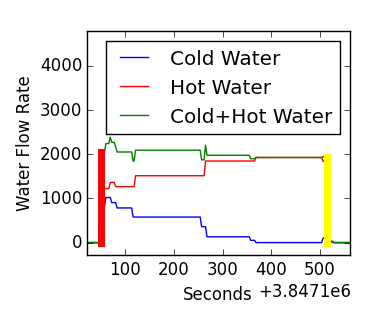
\includegraphics[width=0.5\textwidth]{multidisaggfig/showerFitted.png}&
                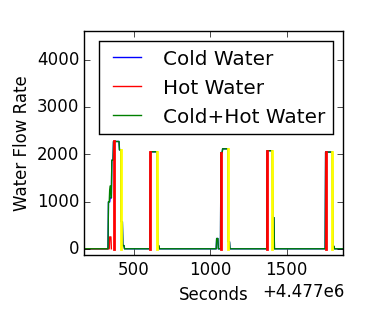
\includegraphics[width=0.5\textwidth]{multidisaggfig/washingMachineWaterFitted.png}\tabularnewline
                (a) & (b)\tabularnewline
                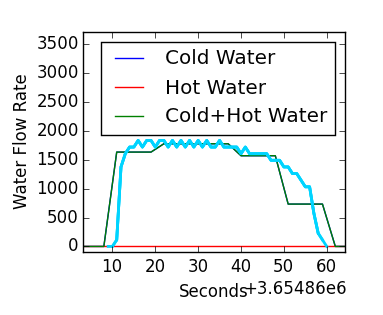
\includegraphics[width=0.5\textwidth]{multidisaggfig/UpToiletFitted.png}&
                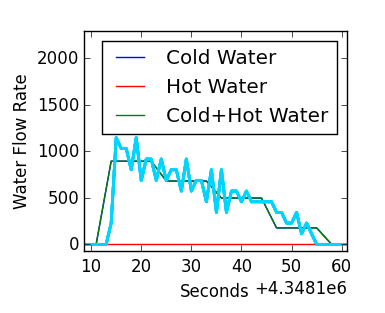
\includegraphics[width=0.5\textwidth]{multidisaggfig/DownToiletFitted.png}
                \tabularnewline
                 (c) & (d)\tabularnewline
                \end{tabular}
                }
        \caption{
        X-axis is the duration to a specific time in seconds, Y-axis is water flow rate in 10000*liter/minute. 
	(a) and (b) denote the water disaggregation of shower and washing machine. The fitted red line denotes the on event of water, and the fitted yellow line denotes the off event of water. 
	(c) and (d) are the disaggregated two toilets of complete usage cycle by dynamic time warping subsequence search. 
	}
        \label{fig_waterDisaggResults}
\end{figure*}
%Figure \ref{fig_waterDisaggResults} (a) and (b) display the water usage of shower and washing machine. 
Applying piecewise motif mining to the water usage lets us disaggregate the
shower and washing machine. %as in Figure \ref{fig_waterDisaggResults} (a) and (b).
The precision, recall and F-measure for the shower disaggregation are 
0.999, 0.972, and 0.986,  
and the precision, recall and F-measure for the washing machine disaggregation are 
0.997, 0.969, and 0.983. 
However, with a variable water flow rate, 
piecewise motif mining has limitations in handling water use ends such as the toilet.
Therefore we use the dynamic time warping subsequence~\cite{rakthanmanon2012searching} search as a complementary to discover these water use ends.  
For the two toilets, we apply dynamic time warping to match the time series.
The water usage results of one toilet, UpToilet, is shown in Figure \ref{fig_dryerResults} (d). 

%There are totally three sinks in the house, namely up sink, down sink and kitchen sink. 
%People may use sinks with only hot water or cold water, or both hot and cold water. 
%The water usage may be large or small. 
%In this case, it is hard to distinguish these three sinks. 
%However, by observing the water usage of up sink and down sink. 
%We find that there's correlation between the down sink and the down toilet, 
%up sink and up toilet. 
%Figure \ref{fig_ToiletSinkCorrelation} (a) and (b) show that the toilet and sink start almost at the same time, 
%or end at the same time. 
We can see that multivariate piecewise motif mining is capable of 
disaggregating water use ends which have sharp on/off water flow rates. 
However, it has limitations in dealing with water use ends with irregular water use patterns, 
such as toilets and sinks. 
Since the water usage of toilets is relatively fixed if used alone, 
some toilet water usages can be disaggregated by using the dynamic time warping subsequence search 
which was researched in \cite{nguyen2013development}. 

